\documentclass[tikz,border=4pt]{standalone}
\usepackage[T1]{fontenc}
\usepackage{newpxtext,newpxmath}
\usepackage{pgfplots}
\pgfplotsset{compat=1.18}
\definecolor{teal}{HTML}{146C78}
\definecolor{orange}{HTML}{CB693F}
\definecolor{ink}{HTML}{203746}
\begin{document}
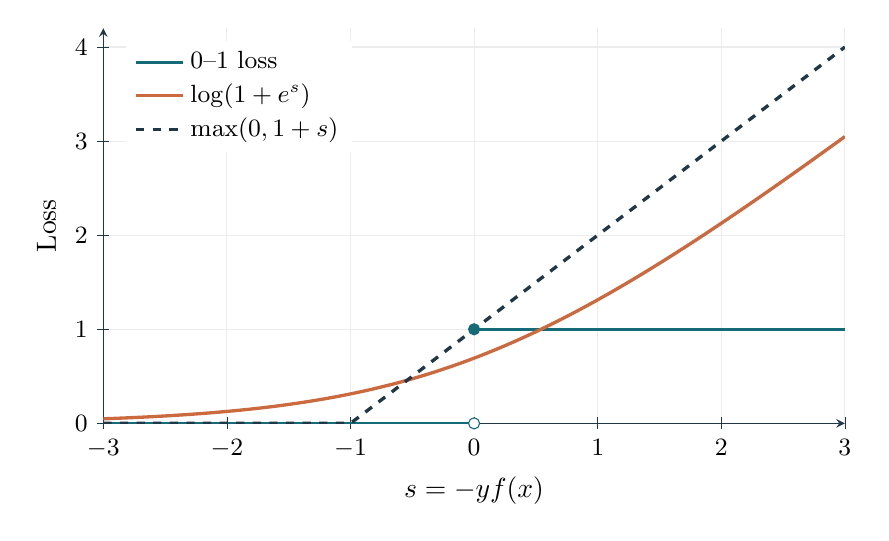
\begin{tikzpicture}
\begin{axis}[
  width=11cm,height=6.6cm,xmin=-3,xmax=3,ymin=0,ymax=4.2,
  xlabel={$s=-y f(x)$},ylabel={Loss},
  axis lines=left,axis line style={ink},
  tick style={ink},ticklabel style={font=\small},
  grid=major,grid style={gray!15},
  legend style={at={(.03,.97)},anchor=north west,draw=none,font=\small},
  legend cell align=left,domain=-3:3,samples=200]
  \addplot[teal,very thick] coordinates {(-3,0) (0,0)};
  \addlegendentry{0--1 loss}
  \addplot[teal,very thick,forget plot] coordinates {(0,1) (3,1)};
  \addplot[teal,only marks,mark=*,mark options={fill=white},forget plot] coordinates {(0,0)};
  \addplot[teal,only marks,mark=*,forget plot] coordinates {(0,1)};
  \addplot[orange,very thick] {ln(1+exp(x))};
  \addlegendentry{$\log(1+e^s)$}
  \addplot[ink,very thick,dashed] {max(0,1+x)};
  \addlegendentry{$\max(0,1+s)$}
\end{axis}
\end{tikzpicture}
\end{document}
